\section{From a chain of seeds to a base-level alignment}
\label{sec:final-alignment-role}

The chaining stage identifies an ordered set of anchors that is plausible at
the scale of genomic coordinates. It does not yet say which bases are
substituted, inserted, or deleted between those anchors. The final-alignment
stage resolves that ambiguity. It refines the ends of a candidate region,
assigns a dynamic-programming score, and, when requested, reconstructs a CIGAR
edit path. In BioSeqDB this is a conditional stage. If an SQL statement needs
only seed-derived coordinates and does not request either CIGAR or exact edit
accounting, \texttt{AlignStage} is disabled. If
\texttt{bioseq.cigar(...)} or an exact \texttt{bioseq.edit(...)} predicate is
present, the stage is enabled and traceback is mandatory.

Calling this operation ``final'' does not imply that every configuration
computes an unconstrained optimum over the whole query and target. KSW2 uses a
finite band and may stop on Z-drop. Block Aligner deliberately explores an
adaptive subset of the matrix. The dedicated GPU route first obtains a
coordinate window from its seeding and chaining stages, then aligns that
window when CIGAR is requested. These are controlled approximations around an
already selected chain. Within the admitted cells, however, the score
recurrences and trace decisions are explicit. When BioSeqDB reports an exact
edit count, it counts substitutions and gaps on the emitted path rather than
using a divergence estimate.

The current CPU implementation exposes two selectable algorithms:

\begin{enumerate}
    \item a Highway port of KSW2, retaining minimap2's single- or
    two-piece-affine recurrence, diagonal-difference representation, banding,
    Z-drop, endpoint selection, and packed CIGAR convention.
    \item a native Highway port of Block Aligner, using a single affine gap
    model, an adaptive block that shifts, grows, and shrinks, and native
    global or X-drop termination.
\end{enumerate}

The generic C++ parameter object selects Block Aligner by default. Its current
in-process block interval is 16--32 cells. The PostgreSQL configuration layer
also selects Block Aligner, but its GUC defaults are still 32--256 and the
custom scan copies those values into the parameter object. This distinction
matters when interpreting the benchmark in
Section~\ref{sec:final-alignment-results}. The source annotation for the
broader tuning grid reports about 22\% lower CPU time for 16--32. The displayed
129\,ms and 172\,ms pair yields a 25.0\% reduction. Neither percentage is
automatically obtained by an unmodified SQL installation using 32--256.

The dedicated all-GPU route adds a third execution contract. Admission
requires the configuration tuple to name Block Aligner, but no CPU Block
kernel runs inside that route. Vulkan seeding and chaining produce coordinate
windows directly. If CIGAR is requested, a separate Vulkan
two-piece-affine CIGAR shader solves those windows. The enum value is thus a
route-admission identity, not evidence that the CPU Block recurrence executed.
BioSeqDB records execution proofs and fails closed so that these two meanings
cannot be silently conflated.

\section{Affine-gap dynamic programming}
\label{sec:final-alignment-affine}

\subsection{Why one gap-open cost is not enough}

Let \(Q=q_1\ldots q_n\) be a query and \(T=t_1\ldots t_m\) a target interval.
Let \(s(q_i,t_j)\) be a substitution score. A linear gap model charges the same
amount for every missing symbol. Biologically, opening a gap and extending an
existing gap are different events. A single insertion of length ten is
usually more plausible than ten independent single-base insertions. An affine
model therefore charges
\[
    g(k) = q + k e,\qquad k\geq 1,
\]
where \(q>0\) is the open penalty and \(e>0\) is the extension penalty. This is
the convention used by minimap2 and BioSeqDB. The first gap symbol costs
\(q+e\).

With target positions on the horizontal axis and query positions on the
vertical axis, a global Needleman--Wunsch--Gotoh recurrence is
\begin{align}
    I(i,j) &= \max\{H(i-1,j)-q-e,\ I(i-1,j)-e\}, \label{eq:affine-i}\\
    D(i,j) &= \max\{H(i,j-1)-q-e,\ D(i,j-1)-e\}, \label{eq:affine-d}\\
    H(i,j) &= \max\{H(i-1,j-1)+s(q_i,t_j),\ I(i,j),\ D(i,j)\}.
    \label{eq:affine-h}
\end{align}
The \(I\) and \(D\) states remember whether the best partial path already ends
in a gap. For global alignment the axes are initialized by cumulative gap
costs. Local alignment additionally permits zero in the maximum. A full
matrix costs \(O(nm)\) time and, if every trace decision is stored,
\(O(nm)\) memory \cite{gotoh_1982_affine}.

BioSeqDB inherits minimap2's default nucleotide scores:
\[
 a=2,\quad b=4,\quad (q_1,e_1)=(4,2),\quad
 (q_2,e_2)=(24,1).
\]
A match scores \(+2\), an ordinary mismatch scores \(-4\), and the two gap
families define
\[
    g(k)=\min\{4+2k,\ 24+k\}.
\]
The short family is strictly cheaper for \(k<20\), the two families tie at
\(k=20\), and the long family is cheaper for \(k>20\). Algebraically, KSW2
maintains two insertion states and two deletion states:
\begin{align}
 I_r(i,j)&=\max\{H(i-1,j)-q_r-e_r,\ I_r(i-1,j)-e_r\},\\
 D_r(i,j)&=\max\{H(i,j-1)-q_r-e_r,\ D_r(i,j-1)-e_r\},
 \qquad r\in\{1,2\},\\
 H(i,j)&=\max\{H(i-1,j-1)+s(q_i,t_j),
 I_1,I_2,D_1,D_2\}.
\end{align}
This two-piece concave cost is important for long reads, where a structural
variant should not be penalized as a series of unrelated short errors.

Block Aligner uses only \((q_1,e_1)\). Its recurrence is therefore not a
drop-in semantic replacement for KSW2 under the default two-piece model. This
is an intentional production trade-off. The adapter projects the short pair,
the block interval, and the X-drop threshold. It does not pretend to honor
the second affine pair, KSW2's band, right-alignment tie flag, end bonus, or
approximate-maximum flag.

\subsection{Banding and Z-drop}

Anchors imply that the desired path should remain near a diagonal. A band of
half-width \(w\) discards cells satisfying
\[
        |i-j| > w
\]
after accounting for the interval's coordinate offset. This changes work from
\(O(nm)\) to approximately \(O(w(n+m))\). The saving is substantial when
\(w\ll \min(n,m)\), but the optimum is lost if a true insertion or deletion
leaves the band. BioSeqDB derives the ordinary alignment width as
\[
        w_{\mathrm{align}}=\lfloor 1.5\,w_{\mathrm{chain}}+1\rfloor.
\]
With the default chaining bandwidth 500, this is 751.

Z-drop supplies a second early-termination rule. Let \(S^\star\) be the best
score seen at \((i^\star,j^\star)\), and let \(S(i,j)\) be the current
anti-diagonal maximum. KSW2 may terminate when both coordinates have advanced
past the best cell and
\begin{equation}
 S^\star-S(i,j)>
 Z+e_z\left|(i-i^\star)-(j-j^\star)\right|.
 \label{eq:zdrop}
\end{equation}
The diagonal-displacement term does not punish a long gap as harshly as an
equal score drop along the same diagonal. In the dual-affine kernel BioSeqDB
uses the long-gap extension penalty \(e_2\) in this test. The default threshold
is \(Z=400\). Block Aligner does not implement Equation~\ref{eq:zdrop}. Its
left and right extensions use the original Block algorithm's X-drop rule and
require two consecutive below-threshold steps before termination.

When an exact SQL edit predicate requires traceable gap fills, the KSW2 path
sets both band and Z-drop to \(-1\) for those mandatory fills. This removes two
sources of premature truncation. It does not turn the whole mapper into a
full-matrix aligner. Seed selection, chain selection, the outer coordinate
window, and any Block configuration remain part of the search contract.

\section{The minimap2 extension strategy and BioSeqDB's port}
\label{sec:final-alignment-three-phase}

\subsection{Three different DP problems, not one matrix}

The current implementation follows the central shape of minimap2's
\texttt{mm\_align1}: extend left of the first seed, fill between seeds, then
extend right of the last seed \cite{minimap2_paper}. These phases have
different endpoint semantics:

\begin{center}
\begin{tabular}{p{0.18\textwidth}p{0.20\textwidth}p{0.23\textwidth}p{0.29\textwidth}}
\toprule
\textbf{Phase} & \textbf{Input orientation} & \textbf{KSW2 contract} &
\textbf{Block contract}\\
\midrule
left extension & reversed subranges & extension-only, right-aligned,
reverse CIGAR, band and Z-drop & native X-drop on directly emitted reversed
compact input\\
seed-to-seed fill & forward & global fill, approximate maximum by default,
two-piece affine & native global adaptive block, single affine\\
right extension & forward & extension-only, band and Z-drop & native X-drop\\
\bottomrule
\end{tabular}
\end{center}

The first and last anchor delimit the inner seeded interval. BioSeqDB expands
an outer interval on either side, bounded by \texttt{max\_gap} and by an
additional score-derived allowance. Left extension is solved in reverse so
that both end extensions can use a forward DP recurrence. Current compact and
lazy sequence views can emit this reversed orientation directly. They do not
first materialize an entire reversed query.

The seed-to-seed walk is especially consequential. A cursor begins at the
first seed. Intermediate anchors whose accumulated query or target distance
is below \texttt{min\_ksw\_len} are skipped without advancing the cursor. Once
both accumulated distances reach the threshold, a global fill is emitted and
the cursor advances. The last anchor always forces the remaining positive
rectangle. With the default threshold 200, a megabase-scale region becomes a
sequence of DP problems often near \(200\times200\), not one
million-by-million matrix. A source-embedded engineering note attributes
roughly a sevenfold total improvement at 903\,kbp to this decomposition. That
number is historical and configuration-specific, but the mechanism remains
in current code.

\begin{figure}[htbp]
\centering
\begin{tikzpicture}[
    x=0.92cm,y=0.92cm,>=Latex,
    seed/.style={circle,fill=black,inner sep=1.7pt},
    phase/.style={rounded corners,draw,fill=blue!7,align=center,
                  minimum height=0.65cm,font=\small},
    lab/.style={font=\small},
    annotation/.style={font=\small,fill=white,text opacity=1,
                       inner xsep=2pt,inner ysep=1.5pt,rounded corners=1pt}
]
  \draw[->,thick] (0,0) -- (12.4,0) node[right,lab]{target coordinate};
  \draw[->,thick] (0,0) -- (0,4.4) node[above,lab]{query coordinate};
  \draw[gray!45,dashed] (0.5,0.5) -- (11.8,4.0);
  \coordinate (a0) at (2.6,1.15);
  \coordinate (a1) at (4.0,1.62);
  \coordinate (a2) at (5.2,2.02);
  \coordinate (a3) at (7.7,2.91);
  \coordinate (a4) at (9.4,3.45);
  \foreach \p in {a0,a1,a2,a3,a4} {\node[seed] at (\p) {};}
  \draw[very thick,teal!70!black] (a0)--(a1)--(a2)--(a3)--(a4);

  \draw[<->,orange!85!black,thick] (0.7,0.65) -- (2.55,1.10);
  \node[phase,anchor=east] at (2.25,0.35) {left extension\\reverse input};

  \draw[<->,purple!75!black,thick] (2.65,1.36) -- (5.15,2.23);
  \node[phase] at (4.0,2.75) {short anchor intervals\\accumulate};

  \draw[<->,purple!75!black,thick] (5.25,2.22) -- (7.65,3.08);
  \node[phase] at (6.6,1.25) {mandatory global\\seed-to-seed fill};

  \draw[<->,orange!85!black,thick] (9.45,3.67) -- (11.5,4.05);
  \node[phase] at (10.35,2.72) {right extension\\forward input};

  \node[annotation,anchor=south east] at (11.85,4.20)
        {$\texttt{min\_ksw\_len}=200$ governs fill boundaries};
\end{tikzpicture}
\caption{BioSeqDB's three-phase region alignment. The drawing reconstructs
the implemented control flow. It is not a copy of a minimap2 figure. Exact
seeds constrain the path, short intervals accumulate, mandatory global fills
resolve gaps, and end extensions refine the outer coordinates.}
\label{fig:three-phase-alignment}
\end{figure}

\begin{algorithm}[htbp]
\caption{Final alignment of one chained region}
\label{alg:three-phase-alignment}
\begin{minipage}{\linewidth}
\small
\textbf{Input.} Query view \(Q\), target view \(T\), ordered anchors \(A\),
and parameters \(P\).
\begin{enumerate}
    \item Derive the inner seed bounds and the bounded outer extension bounds.
    \item Reserve region CIGAR capacity from the outer query and target extents.
    \item If both left outer intervals are non-empty:
    \begin{enumerate}
        \item Run reverse-oriented extension with KSW2 or Block X-drop.
        \item Update the left endpoint from the selected maximum or query-end
              score.
    \end{enumerate}
    \item Set \((q_s,t_s)\gets\) the start of the first seed.
    \item For each later anchor \(a_i\):
    \begin{enumerate}
        \item Set \((q_e,t_e)\gets\) the end coordinates of \(a_i\).
        \item If \(a_i\) is not the last anchor and either
              \(q_e-q_s<P.\textit{minLen}\) or
              \(t_e-t_s<P.\textit{minLen}\), continue without advancing
              \((q_s,t_s)\).
        \item Otherwise, if both accumulated intervals are non-empty, solve
              one mandatory global fill, append its packed CIGAR, and set
              \((q_s,t_s)\gets(q_e,t_e)\).
    \end{enumerate}
    \item If the right outer intervals are non-empty and the selected contract
          permits it, run forward extension and update the right endpoint.
    \item Project reverse-strand query coordinates and final score metadata.
\end{enumerate}
\end{minipage}
\end{algorithm}

Algorithm~\ref{alg:three-phase-alignment} makes the cursor semantics explicit.
The left extension runs only when both outer slices are nonempty. Inside the
anchor loop, skipping a short interval does not advance \((q_s,t_s)\), so
several short intervals accumulate into one mandatory fill. The right
extension then runs only when the selected backend contract permits it.
Reverse-strand projection and final score metadata are applied after these
three phases. This order preserves the chain geometry while allowing KSW2 and
Block Aligner to implement different phase contracts.

\subsection{Where the port intentionally stops matching minimap2}

The inspected minimap2 reference contains more policy than the three boxes in
Figure~\ref{fig:three-phase-alignment}. It handles ignored and tandem seeds,
long-join bandwidth expansion, short-read ungapped shortcuts, splice junction
scores, RNA-specific paths, an approximate first pass followed by
\texttt{mm\_test\_zdrop}, inversion Z-drop, and region splitting after a
dropped gap. The current BioSeqDB path implements the ordinary DNA
seed-to-seed and end-extension core. It does not contain the splice, long-join,
inversion-retry, or second-pass logic in its alignment modules. Consequently,
``minimap2-derived'' is more accurate than ``minimap2-equivalent'' for those
special modes.

The ordinary paths also differ at an anchor boundary. BioSeqDB derives the
boundary from the stored \texttt{cur\_anchor.query\_position} and
\texttt{cur\_anchor.ref\_position}, then adds one. Upstream minimap2 normally
calls \texttt{mm\_adjust\_minier} before extension. Its short-read special path
with homopolymer compression (HPC) disabled is an exception. BioSeqDB does not
perform that adjustment here,
so the DP windows can differ even when the chain anchors agree.

There is also a subtle difference after a dropped phase. KSW2 suppresses the
right extension if a prior phase Z-dropped. The Block path still admits a
right extension because its gap fills are global and its two end extensions
use their own native X-drop domains. This is encoded in the compile-time
algorithm branch rather than hidden in a common KSW-shaped adapter.

\section{KSW2 in BioSeqDB}
\label{sec:final-alignment-ksw2}

\subsection{The Suzuki--Kasahara difference representation}

A straightforward SIMD implementation stores absolute \(H\), \(I\), and \(D\)
scores. Long alignments require wide integers because absolute scores grow with
sequence length. Wide lanes reduce the number of cells processed per vector.
Suzuki and Kasahara observed that neighboring-score differences remain
bounded by the scoring parameters even when the absolute score is large.
KSW2 therefore represents quantities related to
\[
    U(i,j)=H(i,j)-H(i-1,j),\qquad
    V(i,j)=H(i,j)-H(i,j-1),
\]
together with transformed gap offsets. The hot recurrence operates on signed
8-bit partial values. An absolute 32-bit score row is reconstructed only for
exact maximum tracking and endpoints \cite{suzuki_kasahara_2018}.

BioSeqDB ports that organization to Highway. A scalable byte tag supplies the
partial-score lanes, while a scalable 32-bit tag reduces reconstructed maxima.
The source instantiates a single-affine kernel only when
\((q_1,e_1)=(q_2,e_2)\). Under the ordinary defaults the pairs differ, so the
dual-affine kernel is selected. The band is stored by anti-diagonal, and one
direction byte encodes the winning state plus continuation bits for each of
the four gap states.

This representation is \emph{intra-sequence} SIMD: lanes represent cells from
one DP problem. It should not be confused with batching independent sequence
pairs into lanes. The latter was explored separately and is discussed in
Section~\ref{sec:final-alignment-batching}.

\subsection{Endpoint and CIGAR semantics}

KSW2 tracks several endpoint summaries:

\begin{itemize}
    \item the best score and its query/target coordinates.
    \item the best score at the query end, with the associated target
    coordinate.
    \item the best score at the target end, with the associated query
    coordinate.
    \item the bottom-right global score if the band reaches it.
\end{itemize}

Traceback starts from the bottom-right cell for an undropped global fill. For
an extension-only call, reaching the end of the query wins when its score plus
the end bonus exceeds the internal maximum. Otherwise traceback starts at the
best observed cell. Left-extension operations are emitted in reverse and then
reversed back into source order.

The KSW packed representation stores one run as
\[
        \textit{word}=(\textit{length}\ll4)\mid\textit{opcode}.
\]
The shared opcodes are \(0=M\), \(1=I\), \(2=D\), \(3=N\),
\(7={=}\), and \(8=X\). Adjacent equal opcodes are merged both within a
traceback and when fills are appended to a region. A CIGAR such as
\texttt{58M1I33M} is therefore three integers, not 92 per-base records.

\subsection{Port-specific memory and hot-loop changes}

The port is not merely the upstream SSE file wrapped in a module. The current
implementation makes several changes needed by BioSeqDB's data model and
execution engine:

\begin{enumerate}
    \item It accepts an alphabet-generic lazy sequence view. Only the admitted
    subrange is encoded, through the view's \texttt{ptr\_at} slot ring. A
    fragmented or PostgreSQL-backed sequence need not be flattened in advance.
    \item DP state, exact-score rows, encoded scratch, and the backtrack matrix
    live in a per-alignment arena. The returned CIGAR has independent lifetime.
    \item Buffers that are overwritten before first read are not eagerly
    zero-filled. In the dual-affine state, the short and long gap arrays are
    initialized directly to their required offsets. The trace matrix likewise
    skips a full clear.
    \item The common nucleotide scoring layout uses a fused equality-based
    score selection. Generic matrices retain a table path.
    \item Exact anti-diagonal maxima are reduced with Highway 32-bit vectors.
    The same source dispatches to supported x86 and Arm targets.
    \item The single- and dual-affine kernels share one compile-time core,
    removing runtime checks from the inner cell loop.
\end{enumerate}

These changes preserve the KSW2 recurrence and result structure while moving
allocation, encoding, and instruction selection into BioSeqDB's common
infrastructure. They also explain why a comparison with standalone minimap2
must include more than the arithmetic kernel. BioSeqDB saves conversions when
the source is already compact, but pays PostgreSQL, batching, and lazy-view
costs that minimap2 does not have.

\section{Block Aligner: adaptive SIMD dynamic programming}
\label{sec:final-alignment-block}

\subsection{The original algorithm}

Block Aligner starts from the same single-affine recurrence as
Equations~\ref{eq:affine-i}--\ref{eq:affine-h}, but it does not fill a static
band~\cite{block_aligner_paper}. It keeps a square \(B\times B\) block
positioned over the DP matrix. A
step computes only a strip of width \(S\) on the right or bottom edge, where
the reference implementation uses \(S=8\). The next direction is selected by
comparing the first \(S\) scores on the two outgoing borders:
\[
\operatorname{direction}=
\begin{cases}
\mathrm{down},&
\max_{0\le k<S} H(i+B-1,j+k)>
\max_{0\le k<S} H(i+k,j+B-1),\\
\mathrm{right},&\text{otherwise}.
\end{cases}
\]
The block follows the region in which scores appear most promising. Unlike a
static diagonal band, it may drift far from the main diagonal.

Greedy direction selection can be fooled by a long gap or a low-similarity
island. The defining contribution of Block Aligner is therefore adaptive
geometry. When several steps fail to produce a new maximum, it restores a
checkpoint and doubles \(B\). The larger block spans more competing paths. If
a later maximum lies near the suffix of either outgoing border, the block may
halve and advance diagonally. The implementation tests the larger suffix
maximum from the row and column borders. This recovers the speed of a narrow
block in easy regions while retaining a chance of crossing a difficult region.

The original paper reports global, local, and X-drop modes, nucleotide and
protein matrices, and position-specific scoring matrices. Across its chosen
datasets it reports more than five- to tenfold speedups over some comparison
methods with an error rate below 3\% on the evaluated protein and long-read
sets. These are paper results on the authors' hardware and workloads. They are
not BioSeqDB speedups and are not directly comparable with the SQL E2E
measurements below.

\begin{figure}[htbp]
\centering
\begin{tikzpicture}[x=0.48cm,y=0.48cm,>=Latex,font=\scriptsize]
  \def\gridpanel#1{
    \begin{scope}[xshift=#1]
      \draw[step=1,gray!28,very thin] (0,0) grid (8,8);
      \draw[->] (0,0)--(8.5,0) node[right]{$T$};
      \draw[->] (0,0)--(0,8.5) node[above]{$Q$};
      \draw[orange!80!black,very thick] (0,0)--(7.7,7.2);
    \end{scope}
  }

  \gridpanel{0cm}
  \begin{scope}[xshift=0cm]
    \draw[blue!75!black,very thick] (0,0) rectangle (3,3);
    \fill[blue!18] (2,0) rectangle (3,3);
    \fill[purple!18] (0,2) rectangle (3,3);
    \draw[->,thick] (3.1,1.4)--(4.1,1.4);
    \node[align=center] at (4.2,5.9) {\textbf{1. Shift}\\compare \(S\)-score\\border prefixes};
    \node at (1.5,-1.0) {(a) right/down decision};
  \end{scope}

  \gridpanel{5.6cm}
  \begin{scope}[xshift=5.6cm]
    \draw[blue!75!black,very thick] (1,1) rectangle (4,4);
    \draw[teal!75!black,dashed,very thick] (0,0) rectangle (6,6);
    \fill[red!65] (2.7,2.7) circle (0.12);
    \node[red!65!black,anchor=west] at (3.0,2.7) {checkpoint};
    \draw[->,thick] (4.2,4.2)--(5.6,5.6);
    \node[align=center] at (4.5,7.2) {\textbf{2. Grow}\\restore checkpoint\\and double \(B\)};
    \node at (3.0,-1.0) {(b) no new maximum};
  \end{scope}

  \gridpanel{11.2cm}
  \begin{scope}[xshift=11.2cm]
    \draw[teal!75!black,very thick] (0,0) rectangle (6,6);
    \fill[green!25] (4.8,4.8) rectangle (6,6);
    \fill[black] (5.35,5.25) circle (0.12);
    \draw[->,thick] (5.8,5.8)--(7.1,7.1);
    \draw[blue!75!black,dashed,very thick] (3,3) rectangle (6,6);
    \node[align=center] at (3.3,7.3) {\textbf{3. Shrink}\\maximum in border\\suffix};
    \node at (3.0,-1.0) {(c) halve and move diagonally};
  \end{scope}
\end{tikzpicture}
\caption{Reconstruction of the adaptive-block mechanism described by Liu and
Steinegger. A step computes an outgoing strip, growth replays from a saved
checkpoint, and shrinking retains the promising suffix. The orange line
illustrates a possible optimum path. This TikZ drawing was rebuilt from the
algorithm and the paper's Figure~2, not copied from the paper artwork.}
\label{fig:block-adaptive-reconstruction}
\end{figure}

Figure~\ref{fig:block-adaptive-reconstruction} should be read from left to
right. Panel~(a) chooses the next strip from the competing border-prefix
maxima. Panel~(b) restores a checkpoint and enlarges the search after progress
stalls. Panel~(c) halves the block only after a maximum reaches an outgoing
border suffix. The figure therefore depicts an adaptive search trajectory, not
a fixed diagonal band.

\subsection{SIMD inside a block}

Block Aligner lays vectors vertically or horizontally rather than on
anti-diagonals. One gap dependency therefore runs between lanes of the same
vector. For a vector \(x_0,\ldots,x_{L-1}\), the needed prefix operation has
the form
\begin{equation}
    y_i=\max_{0\le k\le i}\{x_k+(i-k)g\},
    \label{eq:block-prefix}
\end{equation}
where \(g=-e\). It is evaluated by shift-and-maximum stages of distances
1, 2, 4, and, for 16 lanes, 8. This takes \(O(\log L)\) vector operations.
A correction carries the last value of the preceding vector into the next
one. The other gap direction and the diagonal transition have ordinary
vector dependencies.

Only four score borders and their checkpoint copies are needed for score
computation, giving \(O(B)\) working score memory. Traceback increases storage
to \(O(B_{\max}(n+m))\) because every computed strip must retain decisions
that the adaptive path may later traverse. A checkpoint also stores the trace
cursor so speculative strips can be discarded when growth replays the region.

\subsection{The current Highway port}

BioSeqDB's implementation is based on
\path{block-aligner-research/src/scan_block.rs}, but it is a native C++26
module rather than a foreign-library call. The production core has the
following concrete geometry:

\begin{itemize}
    \item a fixed step \(S=8\).
    \item signed 16-bit lanes with saturating arithmetic and a bias of
    \(2^{14}\), together with a 32-bit step offset.
    \item a Highway capped tag of at most 16 lanes.
    \item admitted lane counts of exactly 8 or 16, corresponding to the
    proven reference geometries.
    \item power-of-two minimum and maximum block sizes.
    \item global mode for mandatory seed gaps and two-confirmation X-drop for
    left and right extension.
\end{itemize}

At 8 lanes, a shift step is one full vector. At 16 lanes, it is half a
vector. Wider Highway targets are deliberately capped rather than allowed to
change the algorithm's step semantics. An unsupported lane shape, penalty,
coordinate range, matrix layout, or block geometry aborts the selected route.
There is no scalar biological implementation hidden beneath this module. The
16-bit representation is safe for the tuned and tested score and block
geometries. The current runtime contract does not prove a
substitution-score-to-block-size range invariant for every SQL-admitted
configuration. Rejecting unsupported shapes therefore does not by itself prove
that every admitted score and block pairing remains within the tested
saturating-arithmetic range.

The hot rectangle kernel loads a scoring-matrix row once per target column and
reuses it for all query vectors in that column. It computes diagonal,
column-gap, and row-gap candidates, using
Equation~\ref{eq:block-prefix} for the row state. Border arrays are the only
scores written back. Trace masks are compressed with Highway's
\texttt{BitsFromMask}. Two masks are interleaved into a direction word, while
two gap-open and continuation masks are interleaved into a second word. Each
cell therefore contributes four trace bits across two words. This replaces
repeated vector stores followed by scalar bit-shifting.

The traceback itself is a lookup-table state machine over diagonal, row-gap,
and column-gap states. It walks the recorded adaptive strips backward and
accumulates run lengths directly into packed \(M/I/D\) operations. If exact
edit accounting was requested, a diagonal step compares the already resident
padded ranks, while an insertion or deletion contributes one edit. The forward
DP commits the alignment score. The backward trace produces the CIGAR and, when
requested, the exact edit count.

\subsection{BioSeqDB-specific adaptations}

\begin{center}
\small
\begin{tabular}{p{0.20\textwidth}p{0.32\textwidth}p{0.38\textwidth}}
\toprule
\textbf{Aspect} & \textbf{Original Block Aligner} & \textbf{BioSeqDB port}\\
\midrule
Implementation & Rust with explicit SSE2, AVX2, Arm NEON, WebAssembly SIMD and C
bindings & C++26 module with Highway target dispatch and a capped, proven
8/16-lane geometry\\
Input & contiguous sequence or PSSM buffers & alphabet-generic lazy views over
packed, fragmented, or PostgreSQL-backed storage\\
Reverse extension & caller-provided reversed input & direct reverse-oriented
emission from compact storage, with no whole-buffer reverse copy\\
Production modes & global, local, and X-drop are library features & global
seed-gap fill and X-drop end extension only\\
Gap model & single affine, including position-specific variants in the paper
& one generated score matrix and the short minimap2 affine pair\\
Scratch lifetime & library allocation objects & per-alignment BioSeqDB arena,
with bounded subregion encoding\\
Trace & four-bit decisions decoded by a LUT & lane masks compressed with
\texttt{BitsFromMask}, LUT trace, direct packed run construction, optional
edit count\\
Fast exact case & no equivalent resident packed proof & DNA4 packed in 64-bit
words or byte-rank diagonal certificate can bypass DP\\
Route integrity & library call selected by caller & execution proof records
phase, lane width, cells, growth, shrinking, trace, certificate, and forbidden
fallbacks\\
\bottomrule
\end{tabular}
\end{center}

The adapter intentionally omits KSW-only fields. A request that depends on the
second affine pair or KSW tie and endpoint flags must select KSW2. Reusing the
shared \texttt{KswAlignResult} structure is only an output-storage
convenience. It does not make the Block recurrence KSW-compatible.

\subsection{A proof that can avoid the DP entirely}
\label{sec:block-diagonal-certificate}

Many mandatory fills are equal-length and nearly identical. BioSeqDB tests
whether their coordinate diagonal is provably the unique global optimum
before constructing Block scratch. Let the common length be \(n\), let
\[
 D=\sum_{i=1}^{n}s(q_i,t_i)
\]
be the exact coordinate-diagonal score, and let \(M\) be the largest entry in
the admitted generated matrix. Any different global path between equal-length
strings must contain the same positive number \(d\) of inserted and deleted
symbols. It has at most \(n-d\) diagonal pairs and at least one gap run in
each direction. Its score is bounded above by
\[
    (n-d)M-2q-2ed
    \le (n-1)M-2(q+e)=U.
\]
Therefore
\begin{equation}
        D>U
        \quad\Longrightarrow\quad
        \text{the coordinate diagonal is the unique optimum}.
        \label{eq:block-certificate}
\end{equation}
Strict inequality is essential. Equality could expose a different traceback
tie policy.

For resident DNA4 storage packed in 64-bit words, the fast certificate reads
packed two-bit symbols directly, reverses packed groups when required, XORs
query and target, and collapses each two-bit mismatch group for a population count. It computes
the score and, when requested, the edit count without byte expansion. When
CIGAR output is requested, the caller emits one \(nM\) run. A score-only call
does not materialize that run. Its decision is three-valued:

\begin{enumerate}
    \item \emph{not eligible}: no packed scan ran, so the ordinary path,
    including the generic byte certificate, remains available.
    \item \emph{rejected}: exact packed content was scanned but
    Equation~\ref{eq:block-certificate} did not prove uniqueness, so Block DP
    runs with the byte certificate disabled to avoid scanning twice.
    \item \emph{certified}: score and endpoint are committed. A requested edit
    count and requested \(nM\) CIGAR are also committed without constructing
    padded buffers, scratch, or trace. The result CIGAR vector is not allocated
    before the proof succeeds.
\end{enumerate}

This is an exact fast path inside an otherwise heuristic adaptive algorithm.
It does not claim that every Block result is an unconstrained optimum. It
proves one common geometry and delegates all other cases to the normal Block
search.

\subsection{Why fail-closed attestation is part of the algorithm}

Runtime algorithm selection is resolved to a template registry before the hot
loop. For Block Aligner the operation-local proof derives, from immutable
region geometry, how many left, gap, and right calls should be eligible. The
kernel then records how many actually ran, which lane width was used, how many
SIMD vectors and cells were evaluated, whether native X-drop ran, whether the
block grew or shrank, and whether a diagonal certificate replaced DP. The
proof also counts forbidden KSW2 and scalar fallback attempts. A selected
Block route is accepted only if the derived and observed phase counts agree
and all forbidden counters are zero.

This is stronger than logging an enum. It makes a common benchmark error
observable: a test can request a fast backend, encounter an unsupported
shape, and silently measure a slower fallback while still printing the
requested label. BioSeqDB instead aborts that operation. The price is a
narrower admitted contract, but the reported algorithm identity is
falsifiable.

\section{Traceback, CIGAR, and exact edit accounting}
\label{sec:final-alignment-cigar}

The forward score alone cannot explain an alignment. Variant calling,
coordinate projection, and an SQL edit predicate need the path. BioSeqDB uses
one common \texttt{CigarOp} representation after backend-specific traceback:
a 32-bit run length and a 32-bit opcode. KSW2, Block Aligner, and Vulkan all
cross their low-level boundary in KSW's packed
\((\textit{length}\ll4)\mid\textit{opcode}\) form, then append into this
common vector.

Before aligning a region, the CPU path estimates CIGAR capacity from the
outer query and target extents. The reserve hint is capped at
\(4\,\texttt{max\_gap}+64\) operations so a megabase seed span does not
preallocate a gigabyte-scale vector. This cap is a performance hint, not a
semantic maximum. The vector can still grow if a highly alternating path
needs more runs.

There are three cases worth separating:

\begin{enumerate}
    \item A region with several seeds appends the left trace, every mandatory
    fill trace, and the right trace. Adjacent runs with the same opcode merge
    at phase boundaries.
    \item A single-seed region has no seed-to-seed DP rectangle. Its implicit
    seeded interval emits a generic \(M\) run over the common length, followed
    by \(I\) or \(D\) for any length difference.
    \item A certified Block diagonal emits one \(nM\) run without allocating
    trace storage.
\end{enumerate}

The implicit interval in the single-seed case contributes its CIGAR and, when
requested, its exact edit accounting. It does not contribute an implicit seed
score to \texttt{dp\_score}. That field accumulates only actual left, fill, and
right DP calls. The path fields can therefore cover the seeded interval even
when the score field has no corresponding seed contribution.

Block Aligner internally knows whether a diagonal step was an equality or a
mismatch. The common minimap-style ABI deliberately projects \(M\), \(=\), and
\(X\) from Block traceback to generic \(M\). It then coalesces adjacent runs
again so an equality-to-mismatch boundary does not become
\texttt{32M1M}. Exact edit distance must consequently not be inferred by
counting only \(I\) and \(D\) in the displayed Block CIGAR.

When exact edit accounting is requested, Block counts mismatching diagonal
steps during its existing trace. KSW2 reconstructs the same quantity by
walking its packed CIGAR over the clipped query and target ranks. The result is
the unit-cost edit count of the emitted path:
\[
 E_{\mathrm{path}} =
 \#\{\text{unequal diagonal steps}\}
 +\sum_{\mathrm{I\ runs}}\textit{length}
 +\sum_{\mathrm{D\ runs}}\textit{length}.
\]
This count is exact for that path. It should not be confused with the affine
score, where a gap run contributes \(q+ke\), or with seed-derived divergence.
Chapter~8 explains how an exact SQL predicate first uses a safe prefilter and
then applies its strict bound to this traced count.

After alignment, BioSeqDB stores the accumulated DP score as both
\texttt{dp\_score} and the current simplified
\texttt{dp\_max\_score}. It derives block length by summing diagonal and gap
runs. For a Vulkan CIGAR it replays diagonal runs against the packed symbol
arrays to obtain the number of equal symbols, because the shader likewise
emits generic \(M\).

\section{Runtime dispatch and the batched-KSW2 experiment}
\label{sec:final-alignment-batching}

\subsection{Enum outside, templates inside}

PostgreSQL and the C++ API expose a runtime base-alignment selector. The
pipeline registry instantiates a kernel trait for each enum value, dispatches
once, then uses \texttt{if constexpr} inside the region loop. A KSW2 fill does
not test on every cell whether it should have been Block Aligner, and a Block
fill cannot quietly call KSW2. The current internal enum contains:

\begin{center}
\begin{tabular}{lp{0.65\textwidth}}
\toprule
\textbf{Value} & \textbf{Implemented meaning}\\
\midrule
\texttt{KSW2} & Highway intra-sequence single- or dual-affine KSW2\\
\texttt{BLOCK\_ALIGNER} & Highway adaptive-block single-affine alignment\\
\texttt{KSW2\_BATCHED} & deferred fill collection, geometry bucketing,
lane-by-lane KSW2 execution, and ordered restitching\\
\bottomrule
\end{tabular}
\end{center}

The generated PostgreSQL enum omits \texttt{ksw2\_batched}, although the
internal registry still instantiates it. Ordinary SQL users choose KSW2 or
Block Aligner. This omission reflects the true implementation state.

\subsection{What was built for inter-sequence SIMD}

The batched design first converts each left extension, global gap, and right
extension into a descriptor. It records subrange coordinates, strand, phase,
bandwidth, owning region, order within the region, scratch CIGAR, score, edit
count, and final offsets. Descriptors are stably sorted into length brackets
\[
       32,\ 64,\ 128,\ 256
\]
and band brackets
\[
       16,\ 32,\ 64.
\]
Reverse and forward fills are kept separate. A fill with either dimension
above 256 is marked long and routed to ordinary KSW2. After execution,
descriptors are sorted back by region and fill order. CIGARs, scores, edit
counts, and endpoints are stitched into their original chains.

This is useful scheduling infrastructure. It is not yet an inter-sequence
SIMD recurrence. The current function named
\texttt{ksw2\_extz2\_batched\_inner} loops over occupied lanes and calls
\texttt{run\_single\_fill}. That function invokes the ordinary intra-sequence
KSW2 kernel once per lane. Execution evidence deliberately calls them bucket
lanes rather than SIMD DP lanes. The earlier DOC0254 design and some source
comments describe the intended fused-lane endpoint, but current code is
authoritative.

The experiment still yielded two lasting design lessons. First, separating
fill collection from execution is sufficient to expose batch geometry without
changing region semantics. Second, a label such as ``batched'' does not prove
that the arithmetic itself is vectorized across independent sequences.
BioSeqDB's final public CPU choice therefore remains native Block Aligner or
intra-sequence KSW2.

\section{GPU extension and gridded traceback}
\label{sec:final-alignment-gpu}

\subsection{The G3SA idea}

The G3SA extending stage addresses a conflict between the forward pass and
traceback~\cite{g3sa_paper}. GPU forward DP is fastest when scores remain in
registers or shared memory. Conventional traceback wants one direction value
per cell in global memory. Writing that direction matrix can remove the benefit
of the GPU kernel.

G3SA's gridded traceback stores only score states on regularly spaced tile
boundaries. Once the final endpoint is known, the backward kernel loads the
nearest upper-left boundaries, recomputes one tile in fast memory, traces
through that tile, discards its directions, and repeats for the next tile on
the path. Forward memory traffic falls from an entire direction matrix to a
grid of borders. Traceback performs additional arithmetic only in tiles
touched by the final path.

\begin{figure}[htbp]
\centering
\begin{tikzpicture}[x=0.55cm,y=0.55cm,>=Latex,font=\scriptsize]
  \begin{scope}
    \draw[step=1,gray!22,very thin] (0,0) grid (9,9);
    \foreach \x in {0,3,6,9} {
      \draw[blue!65!black,thick] (\x,0)--(\x,9);
    }
    \foreach \y in {0,3,6,9} {
      \draw[blue!65!black,thick] (0,\y)--(9,\y);
    }
    \draw[orange!85!black,very thick]
      (0.1,0.2)..controls (2.2,1.5) and (2.0,3.0)..(3.2,3.2)
      ..controls (5.5,3.6) and (5.2,6.0)..(6.3,6.2)
      ..controls (7.7,7.0) and (8.2,8.1)..(8.9,8.8);
    \node[align=center] at (4.5,10.0)
      {\textbf{Forward pass}\\store only five-state tile borders};
    \node at (4.5,-0.9) {(a) boundary spill};
  \end{scope}

  \begin{scope}[xshift=7.4cm]
    \draw[step=1,gray!22,very thin] (0,0) grid (9,9);
    \foreach \x in {0,3,6,9} {
      \draw[blue!65!black,thick] (\x,0)--(\x,9);
    }
    \foreach \y in {0,3,6,9} {
      \draw[blue!65!black,thick] (0,\y)--(9,\y);
    }
    \fill[purple!18] (6,6) rectangle (9,9);
    \fill[purple!18] (3,3) rectangle (6,6);
    \fill[purple!18] (0,0) rectangle (3,3);
    \draw[orange!85!black,very thick,<-]
      (0.1,0.2)..controls (2.2,1.5) and (2.0,3.0)..(3.2,3.2)
      ..controls (5.5,3.6) and (5.2,6.0)..(6.3,6.2)
      ..controls (7.7,7.0) and (8.2,8.1)..(8.9,8.8);
    \node[align=center] at (4.5,10.0)
      {\textbf{Backward pass}\\recompute one purple tile, trace, discard};
    \node at (4.5,-0.9) {(b) tile-local replay};
  \end{scope}
\end{tikzpicture}
\caption{Reconstruction of gridded traceback from the G3SA mechanism and the
current BioSeqDB Vulkan shader. Blue grid boundaries survive the forward
pass. Purple tiles are recomputed only while the orange path is traced. The
drawing is a new TikZ reconstruction, not copied paper artwork.}
\label{fig:gridded-traceback}
\end{figure}

Figure~\ref{fig:gridded-traceback} separates persisted state from replayed
work. The left panel shows the forward pass spilling only tile-border score
states. The right panel shows traceback recomputing only the purple tiles
touched by the orange path. The design trades extra arithmetic during
traceback for a much smaller forward-pass memory footprint.

G3SA's CUDA implementation uses subwarps, packed bases, anti-diagonal
forward computation, a separate traceback kernel, and a principal grid size
of 64 selected by sensitivity analysis. Its paper reports at most 1.80-fold
end-to-end speedup with one GPU and 6.21-fold with four GPUs over its CPU
baselines. It reports up to 9.73-fold for an individual stage comparison.
Those values describe G3SA's datasets, hardware, and baselines. They motivate
the memory strategy, but they are not evidence about BioSeqDB.

\subsection{BioSeqDB's Vulkan implementation}

BioSeqDB transfers the border-and-recompute idea to Vulkan and to its
PostgreSQL execution boundary. The current dedicated route proceeds as
follows:

\begin{enumerate}
    \item A resident Vulkan minimizer and chaining route emits candidate
    coordinate windows.
    \item If CIGAR is not requested, those coordinate results are returned
    without running the CPU \texttt{AlignStage}.
    \item If CIGAR is requested, the PostgreSQL scheduler packs only each
    selected query and target window into 32-bit symbol ranks. It classifies
    exact, simple-gap, bounded, and gridded jobs.
    \item One Vulkan dispatch solves the batch. Results contain score,
    endpoints, a packed-CIGAR slice, and status. The host verifies every
    slice, replays generic \(M\) against the rank buffers to count equal
    symbols, and constructs the SQL result.
\end{enumerate}

The selected all-GPU tuple is deliberately narrow. Vulkan must be enabled,
GPU seed lookup and the fused frontend must be selected, the target index must
be built on the GPU, minimizer extraction must be the Vulkan minimap-integer
variant, chaining must be Vulkan tiled DP, and the base-alignment selector
must be Block Aligner. Divergence, mapping quality, exact edit filtering, and
the prefilter are excluded from this dedicated tuple. CIGAR additionally
requires \texttt{vulkan\_extend\_enabled}. If any selected component cannot
execute, the statement errors before entering the generic CPU/SIMD pipeline.

The CIGAR shader implements a two-piece-affine global recurrence with five
score states \(H,I_1,I_2,D_1,D_2\). Spans up to 512 symbols use a bounded
full direction matrix. Longer general spans, up to the current 16,384-symbol
admission limit, use a 128-by-128 grid. For a job with tile dimensions
\(b_q,b_t\), the planned traceback capacity in 32-bit words is
\begin{equation}
 \left\lceil\frac{n}{b_q}\right\rceil
 \left\lceil\frac{m}{b_t}\right\rceil
 5\bigl[(b_q+1)+(b_t+1)\bigr]
 +(b_q+1)(b_t+1).
 \label{eq:gpu-trace-capacity}
\end{equation}
The first term stores five states along the bottom and right border of every
tile. The second is one reusable tile-local direction scratch matrix.

The forward invocation visits every tile in row-major order and stores only
those borders. Traceback begins at the bottom-right global endpoint. It
recomputes the containing tile, records source and gap-continuation bits in
the shared scratch slice, walks until it crosses a tile boundary, then
recomputes the next tile. Packed \(M/I/D\) runs are generated backward and
reversed at completion.

Several constrained scripts avoid DP altogether: exact equal-length spans,
one- or two-gap scripts, a bounded unit-gap walk, and a greedy anchored gap
walk. Exact and recognized unit-gap jobs can reserve zero traceback words.
The current caps are 256 symbols for an individual simple gap and 64 gap
operations for the simple-script family.

\subsection{What was inherited and what was not}

\begin{center}
\small
\begin{tabular}{p{0.20\textwidth}p{0.32\textwidth}p{0.38\textwidth}}
\toprule
\textbf{Aspect} & \textbf{G3SA} & \textbf{BioSeqDB}\\
\midrule
Programming model & CUDA kernels integrated with modified minimap2 &
Vulkan compute shaders invoked by a PostgreSQL custom-scan scheduler\\
Forward parallelism & subwarps cooperate on packed anti-diagonal blocks &
current CIGAR shader assigns one scalar DP job to each invocation, relying on
batch-level parallelism\\
Grid size & principal experimental setting 64 & fixed traceback tile length
128 in the current ABI\\
Stored boundary & compact row/column states used by the CUDA kernels & five
two-piece-affine states on each bottom and right tile border\\
Trace endpoint & exact global maximum for full extension, while lightweight
extension greedily tracks an approximate maximum &
bottom-right of the selected global coordinate window in the CIGAR shader\\
Gap model & inspected gridded CUDA trace uses one affine family & two affine
families with short and long gaps\\
Input & packed CUDA query/reference batches & alphabet-rank arrays packed
from lazy/PostgreSQL views after coordinate selection\\
Fast paths & GPU extension kernels and G3SA scheduling optimizations & exact,
simple-script, unit-gap, bounded full-trace, and gridded routes\\
Integration proof & standalone end-to-end aligner comparisons & SQL E2E
counters include selected branch, jobs, waves, CIGAR jobs, traceback words,
declines, and forbidden fallbacks\\
\bottomrule
\end{tabular}
\end{center}

Two current-source limitations prevent an over-broad equivalence claim.
First, invocations within a CIGAR workgroup do not cooperate on one matrix.
The batch is parallel, but each admitted job executes scalar row loops. This
is unlike G3SA's subwarp-level forward kernel. Second, the CIGAR wire carries
band width, Z-drop, and end bonus, but the current bounded and gridded global
CIGAR recurrences use neither Z-drop nor end bonus, and their cell loops do
not prune by the supplied band. Band width is validated at admission. A
separate score-only Vulkan prototype does implement single-affine local
banding for spans up to 512, but that runtime surface is not the same as the
dedicated SQL CIGAR route.

The result is best described as a G3SA-inspired traceback memory layout, not a
Vulkan translation of G3SA. BioSeqDB gains the border/recompute trade-off and
batch amortization, while retaining its own SQL admission rules, alphabet
surface, gap model, result ABI, and fail-closed evidence.

\section{Intermediate measurements and current evidence}
\label{sec:final-alignment-results}

\subsection{CPU block-size sweep}

The current \texttt{Minimap2Params} source preserves a tuning sweep performed
on an Apple M1 with Arm NEON over a long, very-long, and extra-long CCS
benchmark grid. It
used ntHash minimizers and SIMD chaining, with KSW2 reported at 172\,ms for
the cited very-long baseline. Table~\ref{tab:block-sweep} reproduces the
displayed Block timings. The final column is calculated directly from the two
printed millisecond values as \(1-t_{\mathrm{Block}}/172\). It is not copied
from the nearby rounded source annotations, which aggregate the broader grid
and do not always equal the single displayed ratio. In particular, the
displayed 16--32 pair gives 25.0\%, while the broader-grid annotation reports
about 22\%.

\begin{table}[htbp]
\centering
\caption{Historical Block Aligner interval sweep embedded in current source.
Positive reduction means lower time than the displayed 172\,ms KSW2
reference. This was not rerun during thesis drafting.}
\label{tab:block-sweep}
\begin{tabular}{rrr r}
\toprule
\(\boldsymbol{B_{\min}}\) & \(\boldsymbol{B_{\max}}\) &
\textbf{Block time (ms)} & \textbf{Derived reduction}\\
\midrule
32 & 256 & 191 & \(-11.0\%\)\\
32 & 128 & 163 & \(5.2\%\)\\
32 & 64  & 161 & \(6.4\%\)\\
8  & 32  & 139 & \(19.2\%\)\\
8  & 16  & 132 & \(23.3\%\)\\
8  & 64  & 137 & \(20.3\%\)\\
16 & 64  & 135 & \(21.5\%\)\\
16 & 32  & 129 & \(25.0\%\)\\
\bottomrule
\end{tabular}
\end{table}

The trend explains the implementation decision. Most production rectangles in
that workload were short gap fills. A maximum of 256 enlarged eight border and
checkpoint buffers plus the trace geometry even though growth rarely passed
32. The in-process parameter default was therefore changed to 16--32. A
smaller maximum is not universally superior. High-error legacy Oxford
Nanopore reads and long unseeded gaps are exactly the shapes for which Block
growth was designed. PostgreSQL's retained 32--256 defaults are conservative
for those shapes but forgo the measured short-fill win.

The sweep also does not establish score equivalence with KSW2. KSW2 uses two
affine families and a static band. Block uses one affine family and an
adaptive heuristic. A faster time can coexist with a different optimum or a
different placement of a tied gap. Performance and semantic-distance tests
must therefore be reported separately.

\subsection{Resident GPU evidence}

The newest authoritative final-alignment discussion in DOC0356/DOC0357 is the
2026-06-28 signoff addendum over
\path{main/reporting/bioseq_bench_e2e_batch_gpu_proof/report_47.json}.  The
artifact was created at 2026-06-28T00:55:32Z from commit
\texttt{ac58f88500d4ad8652e2}\allowbreak
\texttt{6e163d2840e5713346b4}. Its metadata records
\texttt{dirty=true} and \texttt{fast=false}. Each displayed tuple and case had
one sample, so the timings are scoped signoff observations rather than
variability estimates. The report recorded no rule violations or regressions
and retained nonblocking report-level sanity warnings. Earlier chronological
sections in the documents say that general gridded traceback was incomplete.
The final addenda explicitly supersede those statements, and the current shader
contains the implemented boundary/recompute path.

\begin{table}[htbp]
\centering
\small
\caption{Selected one-sample PostgreSQL E2E evidence from
\texttt{report\_47.json}. ``Gate result'' is the report's case-specific
acceptance measure. All three GPU rows recorded zero CPU fallbacks, zero SIMD
fallbacks, and zero Vulkan declines.}
\label{tab:gpu-alignment-evidence}
\begin{tabular}{p{0.34\textwidth}rrrp{0.20\textwidth}}
\toprule
\textbf{Case} & \textbf{GPU (s)} & \textbf{SIMD (s)} &
\textbf{Speedup} & \textbf{Gate result}\\
\midrule
\texttt{E2E\_BATCH\_512\_MANY\_GAP\_CIGAR}
& 1.241472 & 1.240568 & \(0.999\times\)
& 512 correct matches and 512 fixture-accepted CIGARs\\
\texttt{E2E\_BATCH\_4096\_MANY\_GAP\_CIGAR}
& 1.809468 & 4.511529 & \(2.493\times\)
& 4096 correct matches and 4096 fixture-accepted CIGARs\\
\texttt{E2E\_BATCH\_16\_300M\_SEG\_COORD}
& 10.585378 & 25.746413 & \(2.432\times\)
& 16/16 expected queries found\\
\bottomrule
\end{tabular}
\end{table}

Table~\ref{tab:gpu-alignment-evidence} separates elapsed time from each
fixture's acceptance gate. The 512-job row establishes fixture acceptance
without a speed advantage. The 4096-job row combines the same class of gate
with a \(2.493\times\) ratio. The 300\,Mbp row uses a coordinate-tolerance
gate, not CIGAR-path comparison or row-set parity. These rows therefore cannot
be treated as one uniform equivalence test.

\begin{figure}[htbp]
\centering
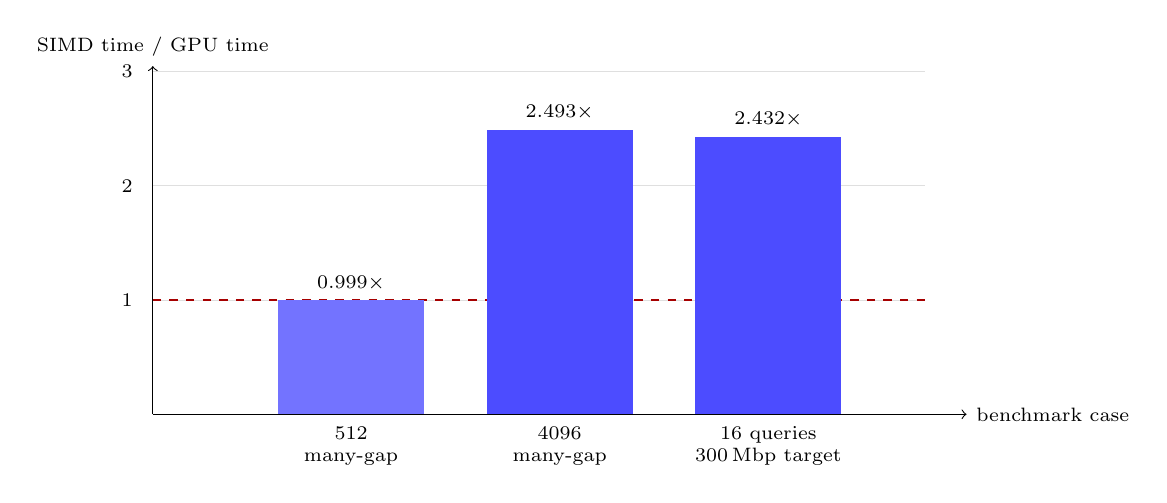
\begin{tikzpicture}[x=2.65cm,y=1.45cm,font=\scriptsize]
  \draw[->] (-0.45,0)--(3.45,0) node[right]{benchmark case};
  \draw[->] (-0.45,0)--(-0.45,3.05) node[above]{SIMD time / GPU time};
  \foreach \y in {1,2,3} {
    \draw[gray!25] (-0.45,\y)--(3.25,\y);
    \node[anchor=east] at (-0.5,\y) {\y};
  }
  \draw[red!65!black,dashed,thick] (-0.45,1)--(3.25,1);
  \fill[blue!55] (0.15,0) rectangle (0.85,0.999);
  \fill[blue!70] (1.15,0) rectangle (1.85,2.493);
  \fill[blue!70] (2.15,0) rectangle (2.85,2.432);
  \node[above] at (0.50,0.999) {\(0.999\times\)};
  \node[above] at (1.50,2.493) {\(2.493\times\)};
  \node[above] at (2.50,2.432) {\(2.432\times\)};
  \node[align=center] at (0.50,-0.28) {512\\many-gap};
  \node[align=center] at (1.50,-0.28) {4096\\many-gap};
  \node[align=center] at (2.50,-0.28) {16 queries\\300\,Mbp target};
\end{tikzpicture}
\caption{Workload-size pattern in the selected E2E evidence. The dashed line
is break-even. A 512-job gridded CIGAR batch is tied, while the two
higher-work cases are consistent with amortization of PostgreSQL and Vulkan
fixed costs. The one-sample cases do not isolate batch size or target size as
the cause.}
\label{fig:gpu-alignment-speedups}
\end{figure}

Figure~\ref{fig:gpu-alignment-speedups} plots the ratio of SIMD time to GPU
time, not either raw duration. A value above one favors the GPU. The 512-job
many-gap case sits at break-even, while the two larger-work cases exceed
\(2.4\times\). The figure is consistent with fixed-cost amortization in these
scoped cases, but it does not establish that explanation causally because the
routes and workloads differ and each case has one sample.

The 4096-job CIGAR case executed 4096 gridded jobs in one extension dispatch
and planned 327,069,696 traceback words. It reduced wall time by 59.891\%.
The 512-job version was correct and used 40,883,712 traceback words, but GPU
and SIMD wall times were effectively equal. This is a useful negative result:
gridded storage alone does not make a small batch fast. Runtime initialization,
rank packing, job classification, allocation, submission, and result
construction remain.

The 300\,Mbp coordinate case gives a different view of amortization. Its GPU
region time was 3.857821\,s versus 25.612293\,s for the SIMD control, a
6.639-fold region speedup. Total wall time improved by 2.432-fold because the
GPU path also spent approximately 12.082\,ms in query sketching,
1547.931\,ms in target deduplication, 785.808\,ms in index building, and
70.653\,ms in seed/chaining runtime. It processed 608 problems in 38 waves,
built 38 segment indexes, and reused them 570 times.

Correctness for that coordinate case means at least one in-tolerance hit for
each of 16 expected queries. It is not exact row-set parity. The GPU tuple
emitted 233 match rows while the SIMD tuple emitted 16. This caveat is
material for downstream SQL that expects one row per query. It does not affect
the 4096-job CIGAR case's reported 4096-of-4096 fixture acceptance, but it
prevents using the coordinate benchmark as a blanket equivalence proof.

The CIGAR fixture gate did not compare the literal GPU CIGAR text, traceback
path, or alignment score with the SIMD result. Its
\texttt{correct\_cigar\_count} required one returned row per query, the expected
strand, a target-coordinate offset below 15 bases, a syntactically valid CIGAR,
and replay that consumed the reported query and target spans. Replay also
validated explicit \(=\) and \(X\) operations. The many-gap fixtures imposed
their own operation constraint, including at least 17 deletion operations.
The table therefore reports fixture-accepted CIGARs, not CIGAR path identity.

Other source-config proof rows in the same report covered 64- and 512-job
long CIGARs, 512- and 4096-job bounded CIGARs, a 4096-job indel case, and an
8192-job bounded case. They reported correct non-empty CIGARs and zero
fallback/decline counters. The final unit and integration gate contained 196
test cases, of which 195 passed and one was skipped, with 3071 of 3071
assertions passing. That contemporaneous gate provides stronger repeatable
correctness coverage than the one-sample benchmark receipt. It proves the
checked-in acceptance matrix, but does not remove the length cap,
scalar-per-job limitation, or row-set caveat.

\subsection{Why the paper and project numbers should not be merged}

The chapter contains four evidence classes that answer different questions.

\begin{table}[htbp]
\centering
\small
\caption{Evidence classes used for final-alignment claims.}
\label{tab:alignment-evidence-classes}
\begin{tabular}{p{0.19\textwidth}p{0.22\textwidth}p{0.25\textwidth}p{0.24\textwidth}}
\toprule
\textbf{Evidence class} & \textbf{Measured scope} &
\textbf{What it supports} & \textbf{What it does not support}\\
\midrule
Block Aligner paper & standalone CPU library on the authors' workloads &
algorithm motivation and published score-error behavior &
BioSeqDB or PostgreSQL speed\\
BioSeqDB M1 sweep & historical integrated CPU tuning with Arm NEON &
the 16--32 in-process Block interval for that workload &
semantic equivalence to KSW2 or the SQL 32--256 default\\
G3SA paper & modified standalone mapper using CUDA &
the border-storage and tile-replay design trade-off &
BioSeqDB Vulkan or SQL performance\\
BioSeqDB report 47 & one-sample dirty PostgreSQL E2E signoff &
case-scoped route execution, acceptance gates, and elapsed times &
algorithm-only speed, literal CIGAR identity, or row-set parity\\
\bottomrule
\end{tabular}
\end{table}

Table~\ref{tab:alignment-evidence-classes} prevents a single ``alignment
speedup'' column from collapsing incompatible scopes. The Block paper isolates
a library algorithm. The M1 sweep chooses CPU scratch geometry. G3SA measures
a CUDA mapper. Report 47 includes PostgreSQL planning, data preparation, target
index handling, batching, GPU submission, and SQL projection. Each number is
used only for the design decision that its evidence class supports.

\section{The final solution and its boundaries}
\label{sec:final-alignment-decision}

\subsection{What was retained}

The resulting architecture is a portfolio with explicit route contracts,
rather than one kernel forced onto every query:

\begin{enumerate}
    \item The region geometry remains minimap2-derived. Left extension,
    accumulated seed-gap fills, and right extension preserve the useful
    decomposition that prevents enormous DP matrices.
    \item KSW2 remains the semantic reference option for two-piece-affine
    scoring, finite bands, Z-drop, and minimap-style endpoint selection. The
    BioSeqDB port adds lazy subrange encoding, arena allocation, eliminated
    clears, and portable Highway dispatch.
    \item Native Block Aligner is the default CPU selection. It is favored for
    the many short mandatory fills exposed by the seed walk. The implementation
    adds direct compact input, compressed trace masks, fused edit counting,
    exact diagonal certificates, and fail-closed phase evidence.
    \item Batched KSW2 retains descriptor collection, geometry grouping, and
    deterministic restitching as an internal experiment. It is not exposed as
    a generated PostgreSQL GUC because its arithmetic remains lane-by-lane.
    \item The optional dedicated GPU tuple uses resident Vulkan seeding and
    chaining. Its CIGAR route applies a G3SA-inspired 128-cell border/recompute
    scheme with a BioSeqDB-specific two-piece-affine shader and SQL evidence.
\end{enumerate}

\begin{table}[htbp]
\centering
\small
\caption{Current final-alignment selection rules. ``Default'' is stated at
the layer where it is actually defined.}
\label{tab:final-alignment-selection}
\begin{tabular}{p{0.20\textwidth}p{0.21\textwidth}p{0.25\textwidth}p{0.24\textwidth}}
\toprule
\textbf{Route} & \textbf{How selected} & \textbf{Best reason to select} &
\textbf{Main limitation}\\
\midrule
CPU Block & C++ and PostgreSQL base-alignment default & many short fills,
portable SIMD, low scratch at tuned block sizes & single affine and adaptive
heuristic. C++ 16--32 and SQL 32--256 defaults differ\\
CPU KSW2 & explicit base-alignment option & two-piece affine, band/Z-drop,
closest current path to minimap2's ordinary extension core & missing
minimap2 splice, inversion, and second-pass policies in the surrounding port\\
internal batched KSW2 & internal enum only. Generated SQL value omitted &
experimentation with deferred fill scheduling and restitching & no fused
inter-sequence SIMD DP yet\\
dedicated Vulkan & complete all-GPU tuple, plus explicit extension enable for
CIGAR & sufficiently large batches or targets, resident index reuse, gridded
CIGAR memory & narrow SQL feature tuple, 16,384-symbol CIGAR span cap,
scalar-per-job DP, no band/Z-drop in current CIGAR recurrence\\
no base DP & neither CIGAR nor exact edit requested & avoid work when
seed/chain coordinates satisfy projection needs & no base-level path or exact
edit result\\
\bottomrule
\end{tabular}
\end{table}

Table~\ref{tab:final-alignment-selection} shows that ``default'' is
layer-specific. CPU Block is the C++ and PostgreSQL base-alignment default, but
that choice does not force the dedicated Vulkan route. KSW2 remains available
when its two-piece-affine and endpoint semantics matter. The no-base-DP row is
valid only when neither CIGAR nor an exact edit count is requested. Route
selection therefore depends on requested outputs and admitted geometry, not
only on the backend name.

\subsection{How the final design differs from the starting point}

The starting point was conceptually simple: port minimap2's KSW2 calls and
obtain a CIGAR. The final design differs at every surrounding boundary.
Sequences are not eagerly converted whole. A chain is split into accumulated
mandatory fills. The kernel is selected once and compiled into a branch-free
inner path. Block Aligner is not disguised behind all KSW flags. Traceback can
produce the exact SQL edit count. A packed diagonal proof can eliminate DP.
Algorithm execution is attested. A GPU route owns its whole selected
seed--chain--coordinate--CIGAR path and is forbidden from falling back.

The changes also reveal which optimizations did \emph{not} become the final
solution. The first idea of inter-sequence KSW2 batching stopped at scheduling
and stitching. A Block interval of 32--256 was too expensive for the measured
short-fill CPU workload, although it remains the SQL safety-oriented default.
The first bounded GPU CIGAR route was insufficient for long many-gap cases,
which motivated gridded traceback. Even after gridded traceback, 512 jobs did
not beat SIMD because fixed costs dominated. The final system therefore
retains multiple routes and reports the break-even behavior instead of
declaring one accelerator universally faster.

\subsection{Open technical limitations}

Four limitations define useful future work:

\begin{enumerate}
    \item \textbf{Semantic modes.} The BioSeqDB minimap2 port needs explicit
    splice/RNA, long-join, inversion, and two-pass Z-drop support before those
    minimap2 modes can be claimed. Block Aligner would need a two-piece-affine
    extension, or a documented routing rule back to KSW2, for closer default
    score compatibility.
    \item \textbf{Configuration convergence.} The 16--32 C++ tuning choice and
    32--256 PostgreSQL GUC defaults should be reconciled through an
    error-profile-aware policy. A single hard-coded interval is unlikely to be
    optimal for both high-accuracy CCS and noisy legacy reads.
    \item \textbf{True inter-sequence parallelism.} The descriptor buckets in
    KSW2-batched and the Vulkan CIGAR job batch are scheduling parallelism.
    A fused CPU lane recurrence or cooperative Vulkan tile would add arithmetic
    parallelism within one dispatch.
    \item \textbf{GPU parity and endpoint policy.} The CIGAR shader should
    either implement its admitted band, Z-drop, and endpoint fields or remove
    them from that wire contract. Exact emitted row-set parity should be added
    to the 300\,Mbp E2E gate, not inferred from one correct hit per query.
\end{enumerate}

The central conclusion is therefore narrower and more useful than ``GPU DP is
fast'' or ``Block Aligner replaces KSW2''. BioSeqDB makes final alignment a
query-dependent, inspectable execution stage. It preserves KSW2 where its
two-piece-affine and endpoint semantics are required, uses native Block
geometry for the measured short-fill CPU regime, and admits a gridded Vulkan
route only for a complete, fail-closed GPU statement shape. CIGAR, edit
distance, score, route identity, and benchmark scope remain separate pieces
of evidence. That separation is what allows a database-resident mapper to
evolve without hiding algorithmic changes behind one SQL function name.

The exposition now steps back by one runtime stage. Final alignment was
described first so that its scoring semantics, cost, and exact edit result are
available when judging a cheaper rejection procedure. In the executed
pipeline, however, the prefilter in the next chapter lies between chaining and
this alignment stage. It may eliminate work only within a proved safe domain.
Every surviving region still follows the alignment and exact post-filter
contracts established above.
